\subsection{Capacitores}

\subsubsection{Definición de capacitor}

Un \textbf{capacitor}, también conocido como \textbf{condensador}, es un componente eléctrico pasivo que tiene la capacidad de \textbf{almacenar energía en forma de un campo eléctrico}. Está compuesto por dos conductores (llamados placas) separados por un material dieléctrico, que actúa como aislante.

Cuando se aplica una diferencia de potencial entre las placas, una de ellas acumula carga positiva y la otra carga negativa, generando así un campo eléctrico entre ellas (ver figura \ref{fig:capacitor_charge}). La capacidad del capacitor para almacenar carga depende de sus características físicas y del dieléctrico utilizado.

La capacitancia \( C \) de un capacitor se define como la razón entre la magnitud de la carga almacenada en una de sus placas (\( Q \)) y la diferencia de potencial (\( \Delta V \)) entre las placas:
\begin{equation}
    C = \frac{Q}{V}
    \label{eq:capacitance}    
\end{equation}
donde:
\begin{itemize}
    \item \( C \) es la \textbf{capacitancia} del capacitor, medida en faradios (\(\si{\farad}\)) (siempre es una cantidad positiva).
    \item \( Q \) es la \textbf{carga eléctrica} almacenada en una de las placas del capacitor, medida en coulombs (\(\si{\coulomb}\)).
    \item \( V \) es la \textbf{diferencia de potencial} entre las placas del capacitor, medida en voltios (\(\si{\volt}\)).
\end{itemize}

\begin{figure}[ht]
    \centering
    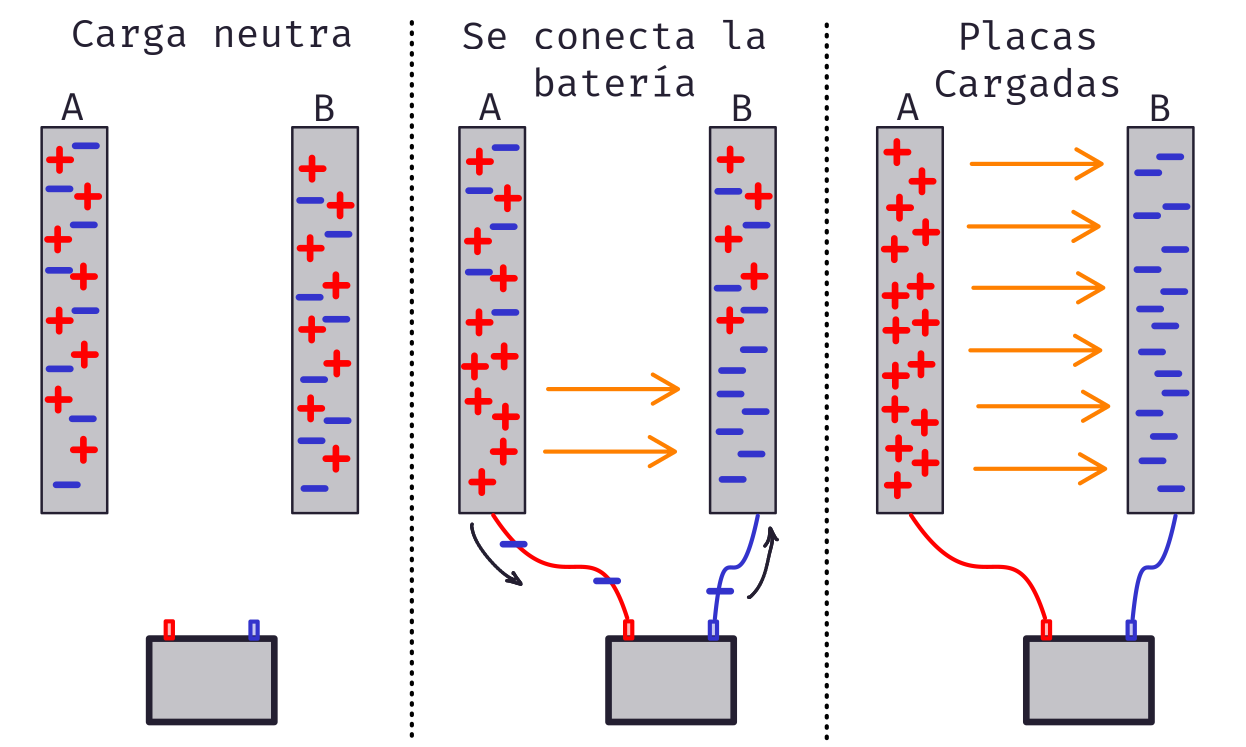
\includegraphics[width=0.7\textwidth]{capacitor_charge.png}
    \caption{Las cargas negativas fluyen de una placa a la otra.}
    \label{fig:capacitor_charge}
\end{figure}

Un faradio es una unidad muy grande, por lo que en la práctica suelen utilizarse submúltiplos como el microfaradio (\(\mu\si{\farad}\)), nanofaradio (n\(\si{\farad}\)) o picofaradio (p\(\si{\farad}\)).

\paragraph{Premisas y consideraciones importantes:}

La definición \( C = Q/\Delta V \) asume que las placas tienen cargas iguales y opuestas (\( +Q \) y \( -Q \)). Si el capacitor está desbalanceado, la capacitancia no puede calcularse directamente con esta fórmula, pues el sistema ya no es un capacitor ideal.

\subsubsection{Geometría de los conductores}

La capacitancia no depende de \(Q\) ni de \(\Delta V\), sino de la geometría del capacitor y del material dieléctrico entre sus placas.

\paragraph{1. Capacitor de placas planas paralelas}

Por ejemplo si se tienen \hl{placas paralelas} de depende de factores como el área de las placas (\(A\)), la distancia entre ellas (\(d\)) y la permitividad del dieléctrico (\( \varepsilon_0 \) para el vacío) según la siguiente fórmula:

\[
C = \varepsilon_0 \frac{A}{d}
\]

donde:
\begin{itemize}
    \item \( \varepsilon_0 \) es la \textbf{permitividad} del material dieléctrico entre las placas (vacío), que se define como la capacidad de un material para almacenar carga eléctrica en un campo eléctrico. Se mide en faradios por metro (\(\si{\farad\per\meter}\)).
    \item \( A \) es el área de una de las placas del capacitor, medida en metros cuadrados (\(\si{\meter\squared}\)).
    \item \( d \) es la distancia entre las placas, medida en metros (\(\si{\meter}\)).
\end{itemize}

Cuando la \hl{geometría de los conductores} es distinta a la de un capacitor de placas planas y paralelas, la expresión de la capacitancia cambia, aunque el principio físico fundamental sigue siendo el mismo: almacenar energía en forma de campo eléctrico entre conductores separados por un dieléctrico.

\paragraph{2. Capacitor esférico}

Consiste en dos esferas concéntricas de radios \( R_1 \) (interna) y \( R_2 \) (externa). Su capacitancia es:

\[
C = 4\pi \varepsilon_0 \frac{R_1 R_2}{R_2 - R_1}
\]

\paragraph{3. Capacitor cilíndrico}

Está formado por dos cilindros coaxiales, uno de radio interno \( a \) y otro de radio externo \( b \), y de longitud \( L \) (suponiendo \( L \gg b \)). La capacitancia es:

\[
C = \frac{2\pi \varepsilon_0 L}{\ln(b/a)}
\]

\paragraph{4. Geometrías irregulares o generales}

En geometrías más complejas, la capacitancia no puede obtenerse de forma analítica sencilla. En estos casos se recurre a:

\begin{itemize}
    \item Métodos numéricos
    \item Aproximaciones analíticas
    \item Medición experimental
\end{itemize}

Cuando se cambia la geometría, ya no es válida la fórmula simple \( C = \varepsilon_0 \frac{A}{d} \). Es necesario \textbf{considerar la distribución del campo eléctrico} que surge de la nueva disposición geométrica, y calcular la capacitancia a partir de las definiciones fundamentales, como:

\[
C = \frac{Q}{V}
\]
donde \( V \) ahora debe calcularse usando la ley de Gauss o integrando el campo eléctrico apropiado para la geometría dada.

\subsubsection{Energía almacenada en un capacitor}

La fórmula de la energía almacenada en un capacitor,

\begin{equation}
    U = \frac{1}{2} QV
\end{equation}
puede demostrarse considerando el trabajo necesario para cargar el capacitor, es decir, para mover carga desde una placa a la otra en contra del campo eléctrico generado.

\paragraph{Demostración}

Supongamos que inicialmente el capacitor no tiene carga. Para cargarlo, se debe transferir carga desde una placa hacia la otra (esto lo realizará una batería). En un instante cualquiera, si la carga acumulada es \( q \), la diferencia de potencial entre las placas es:

\[
V(q) = \frac{q}{C}
\]

Para mover una carga diferencial \( dq \) contra esta diferencia de potencial, se debe realizar un trabajo diferencial:

\[
dW = V(q) \, dq = \frac{q}{C} \, dq
\]


Entonces, el trabajo total \( W \) para cargar el capacitor desde \( q = 0 \) hasta \( q = Q \) es:

\[
W = \int_{0}^{Q} \frac{q}{C} \, dq = \frac{1}{C} \int_{0}^{Q} q \, dq = \frac{1}{C} \cdot \frac{Q^2}{2} = \frac{1}{2} \frac{Q^2}{C}
\]

Ese trabajo realizado es la energía almacenada en el campo eléctrico del capacitor, por lo tanto:

\[
U = \frac{1}{2} \frac{Q^2}{C}
\]

Como \( Q = CV \), podemos reemplazar en la expresión para obtener las otras formas equivalentes de la energía:

- En función de \( Q \) y \( V \):

\[
U = \frac{1}{2} QV
\]

- En función de \( C \) y \( V \):

\[
U = \frac{1}{2} CV^2
\]

Estas tres expresiones son equivalentes, y se utilizan según las variables conocidas en un problema.

\textbf{Interpretación física:} La energía \( U \) no está en la carga como tal, sino en el campo eléctrico que se establece entre las placas del capacitor. Esta energía puede recuperarse, por ejemplo, al descargar el capacitor en un circuito.

\subsubsection{Dieléctrico en un capacitor}

El dieléctrico es un material aislante que se coloca entre las placas de un capacitor. Su función principal es modificar el campo eléctrico dentro del capacitor y, como consecuencia, aumentar su capacitancia sin necesidad de cambiar su geometría.

\paragraph{¿Qué hace un dieléctrico?}

\begin{figure}[ht]
    \centering
    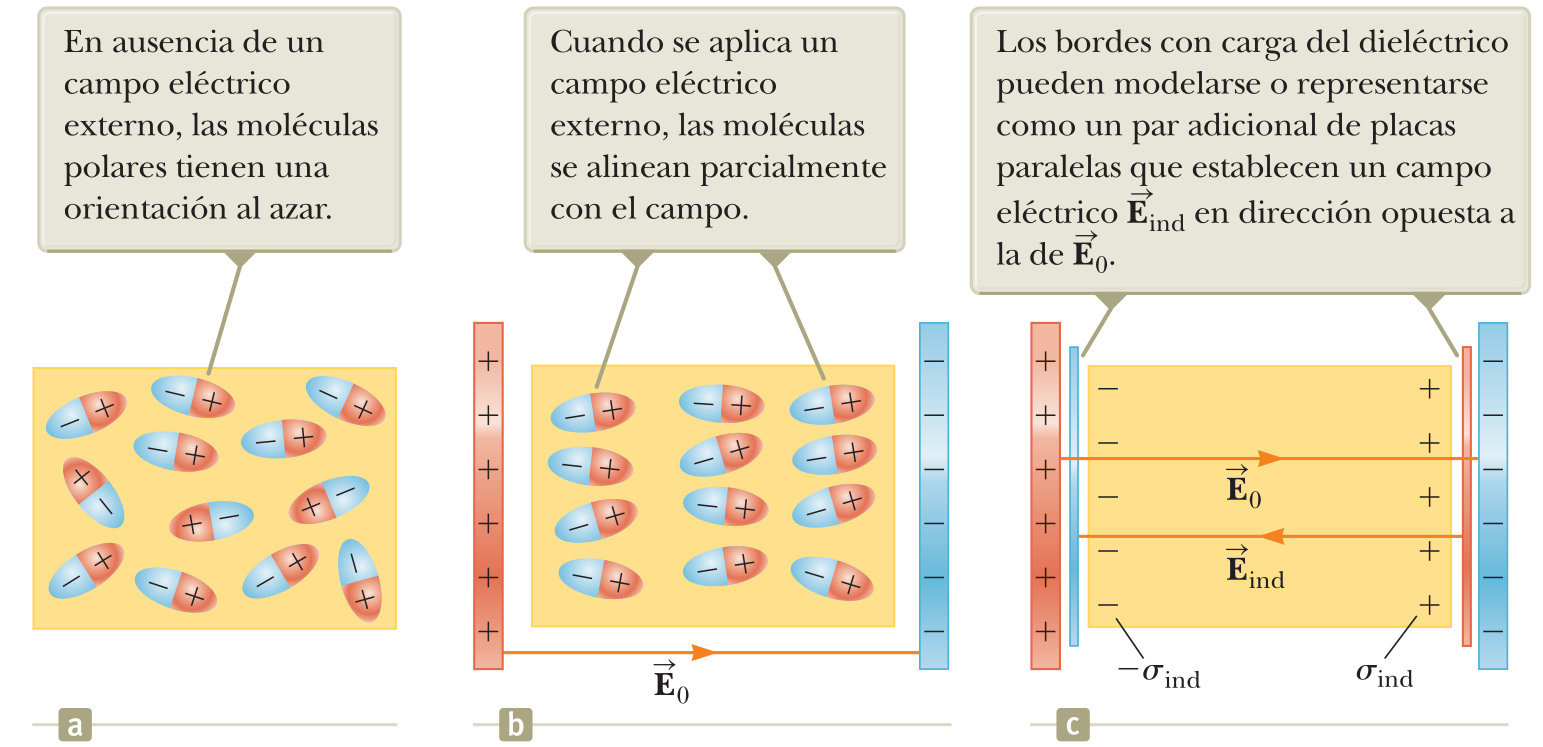
\includegraphics[width=0.8\textwidth]{capacitor_dielectric.png}
    \caption{Polarización de un dieléctrico en un capacitor.}
    \label{fig:capacitor_dieletrico}
\end{figure}
Cuando se introduce un dieléctrico entre las placas de un capacitor:
\begin{enumerate}
    \item Se polariza: Las moléculas del dieléctrico se alinean parcialmente con el campo eléctrico, creando campos eléctricos internos opuestos al campo aplicado.
    \item Reduce el campo eléctrico efectivo entre las placas.
    \item Esto implica que, para una misma cantidad de carga \( Q \), la diferencia de potencial \( V \) disminuye.
    \item Como \( C = \frac{Q}{V} \), una menor \( V \) implica una mayor capacitancia.
\end{enumerate}
\newpage
\paragraph{Permitividad relativa \( \varepsilon_r \)}

El efecto del dieléctrico se caracteriza mediante una constante adimensional llamada permitividad relativa o constante dieléctrica, denotada por:

\[
\varepsilon_r = \frac{\varepsilon}{\varepsilon_0}
\]

\begin{itemize}
    \item \( \varepsilon_r \) es la permitividad relativa del material dieléctrico.
    \item \( \varepsilon \) es la permitividad del material dieléctrico.
\end{itemize}

Algunas bibliografias utilizan la letra ``k'' cursiva (\textit{k}) para referirse a la constante dieléctrica, aunque usar \( \varepsilon_r \) evita confusión con la constante \(k\) d\textsl{}e la ley de Coulomb.

Cuando se introduce un dieléctrico completamente entre las placas, la capacitancia del capacitor se modifica de:

\[
C_0 = \varepsilon_0 \frac{A}{d}
\quad \text{(sin dieléctrico)}
\]

a:

\[
C = \varepsilon_0 \varepsilon_r \frac{A}{d} = \varepsilon \frac{A}{d}
\quad \text{(con dieléctrico)}
\]

Por lo tanto:

\begin{equation}
    \boxed{C = \varepsilon_r C_0}
    \label{eq:capacitance_dielectric}
\end{equation}

Esto significa que la capacitancia aumenta en un factor \( \varepsilon_r \), que típicamente está entre 2 y 10 para muchos materiales comunes, aunque puede ser mucho mayor en materiales especiales.

\paragraph{Energía almacenada con dieléctrico}

La energía también cambia dependiendo de cómo se conecta el capacitor:

\textbf{Caso 1: } el capacitor está desconectado de la fuente y se inserta el dieléctrico:
\begin{itemize}
    \item \( Q \) se mantiene constante (esta desconectado de la fuente).
    \item \( V \) disminuye (por el campo opuesto del dielectrico).
    \item \( C \) aumenta.
    \item La energía disminuye: parte de la energía se transfiere al dieléctrico como trabajo de polarización.
\end{itemize}

\[
U = \frac{1}{2} \frac{Q^2}{C} \quad \text{(disminuye porque } C \text{ aumenta)}
\]

\textbf{Caso 2: } el capacitor está conectado a una fuente constante \( V \) al insertar el dieléctrico:
\begin{itemize}
    \item \( V \) se mantiene constante.
    \item \( Q \) aumenta (la fuente compensa la disminución de \( V \)).
    \item \( C \) aumenta.
    \item La energía almacenada aumenta, y esta energía adicional proviene de la fuente de voltaje.
\end{itemize}

\[
U = \frac{1}{2} C V^2 \quad \text{(aumenta porque } C \text{ aumenta)}
\]

\paragraph{Resumen de efectos del dieléctrico}

El dieléctrico tiene varios efectos importantes en un capacitor:
\begin{itemize}
    \item Aumenta la capacitancia (\( C \)).
    \item Reduce el campo eléctrico (\( E \)) entre las placas.
    \item Almacena energía adicional en forma de polarización.
    \item Modifica la energía almacenada (\( U \)).
    \item Cambia la expresión de capacitancia (\( C \)) dependiendo de si el capacitor está conectado a una fuente o no.
\end{itemize}

\subsubsection{Potencial o Voltaje de ruptura de un dieléctrico}

El voltaje de ruptura (también llamado tensión de ruptura o dieléctrica) es la máxima diferencia de potencial que puede aplicarse entre las placas de un capacitor (o entre dos puntos de un aislante) antes de que el material dieléctrico falle y se vuelva conductor.

\paragraph{¿Qué ocurre cuando se supera el voltaje de ruptura?}

Cuando el campo eléctrico en el dieléctrico supera un valor crítico, llamado intensidad de campo de ruptura (o rigidez dieléctrica), el material se ioniza, es decir, sus átomos o moléculas pierden electrones debido al campo intenso, y se produce una descarga eléctrica: el dieléctrico pierde su capacidad aislante y permite el paso de corriente.

Esto puede generar:

\begin{itemize}
    \item Chispas o arcos eléctricos.
    \item Daño permanente al capacitor.
    \item Cortocircuitos en circuitos eléctricos.
\end{itemize}

\paragraph{Campo eléctrico de ruptura \( E_{\text{ruptura}} \)}

Se expresa como:

\[
E_{\text{ruptura}} = \frac{V_{\text{ruptura}}}{d}
\]
donde:
\begin{itemize}
    \item \( V_{\text{ruptura}} \) es el voltaje de ruptura.
    \item \( d \) es la distancia entre las placas del capacitor.
    \item \( E_{\text{ruptura}} \) es la intensidad de campo eléctrico de ruptura, medida en voltios por metro (V/m) o más comúnmente en megavoltios por metro (MV/m).
\end{itemize}

\subparagraph{Valores típicos de \( V_{\text{ruptura}} \)}

\begin{table*}[ht]
    \centering
    \begin{tabular}{|c|c|c|}
        \hline
        \textbf{Material} & \textbf{Constante dieléctica \(\varepsilon_r\)} & \textbf{Resistencia}\\ 
        &&\textbf{de ruptura (MV/m)} \\
        \hline
        Aire & 1.00059 & 3 \\
        Papel impregnado & 3.5 & 11 \\
        Nylon & 3.4 & 14 \\
        Polietileno & 2.56 & 24 \\
        Teflón & 2.1 & 60 \\
        \hline
    \end{tabular}
    \caption{Valores típicos de tensión de ruptura para diferentes dieléctricos.}
    \label{tab:ruptura}
\end{table*}

\subsubsection{Capacitores en serie y paralelo}

Los capacitores pueden conectarse en serie o en paralelo, y la forma en que se conectan afecta la capacitancia total del circuito.

\paragraph{1. Capacitores en paralelo}

\begin{figure}[ht]
    \centering
    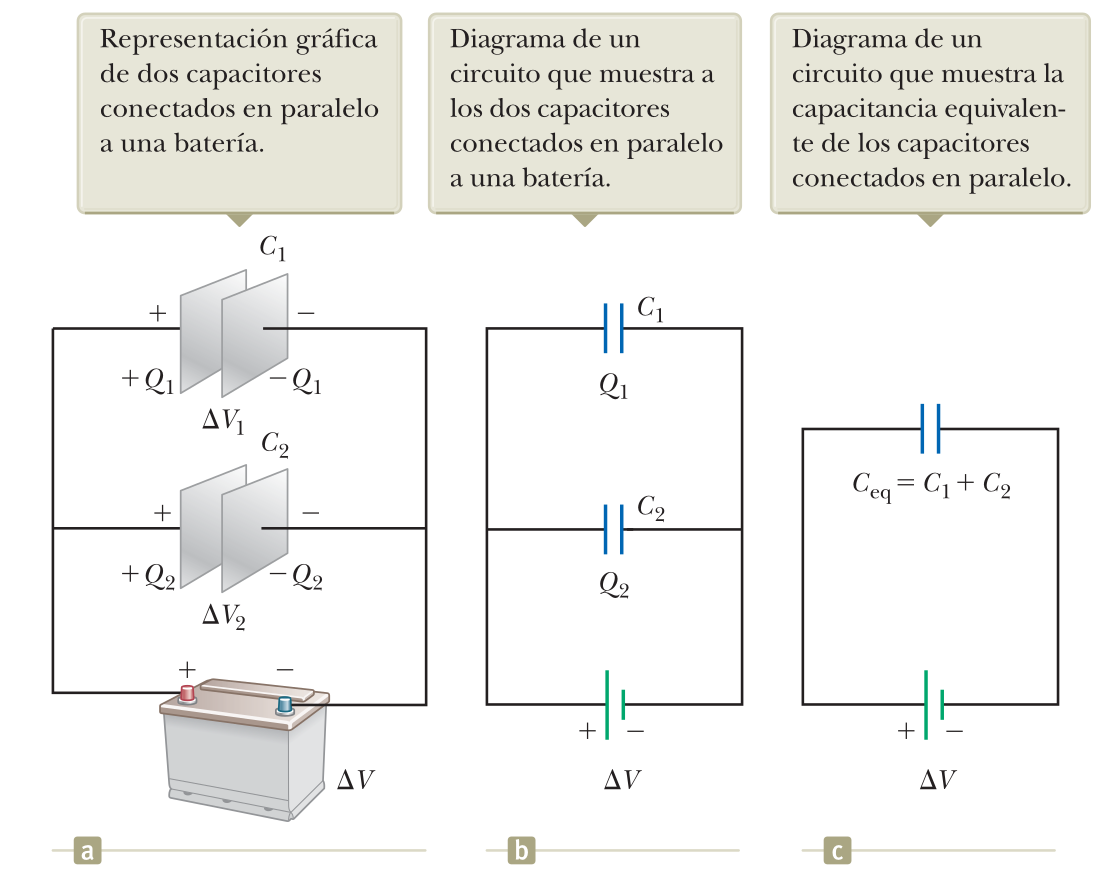
\includegraphics[width=0.8\textwidth]{capacitors_parallel.png}
    \caption{Configuración de capacitores en paralelo.}
    \label{fig:capacitors_parallel}    
\end{figure}

\textbf{Configuración:} Todos los capacitores están conectados a la misma diferencia de potencial \( V \). Es decir:

\[
V_1 = V_2 = \dots = V_n = V
\]

\textbf{Carga total:} La carga total almacenada es la suma de las cargas individuales:

\[
Q_{\text{total}} = Q_1 + Q_2 + \dots + Q_n
\]

Como \( Q_i = C_i V \), entonces:

\[
Q_{\text{total}} = C_1 V + C_2 V + \dots + C_n V = \left( C_1 + C_2 + \dots + C_n \right) V
\]

Pero, por definición:

\[
Q_{\text{total}} = C_{\text{eq}} V
\]

Comparando ambas expresiones:

\[
C_{\text{eq}} = C_1 + C_2 + \dots + C_n
\]

\textbf{Resultado:} La capacitancia equivalente en paralelo es la suma directa de las capacitancias individuales.

Cuando los capacitores están conectados en paralelo, la capacitancia total \( C_{\text{total}} \) se calcula sumando las capacitancias individuales:
\begin{equation}
    \boxed{C_{\text{total}} = C_1 + C_2 + C_3 + \ldots}
    \label{eq:capacitance_parallel}
\end{equation}
donde \( C_1, C_2, C_3, \ldots \) son las capacitancias individuales de los capacitores conectados en paralelo.

\paragraph{2. Capacitores en serie}

\begin{figure}[ht]
    \centering
    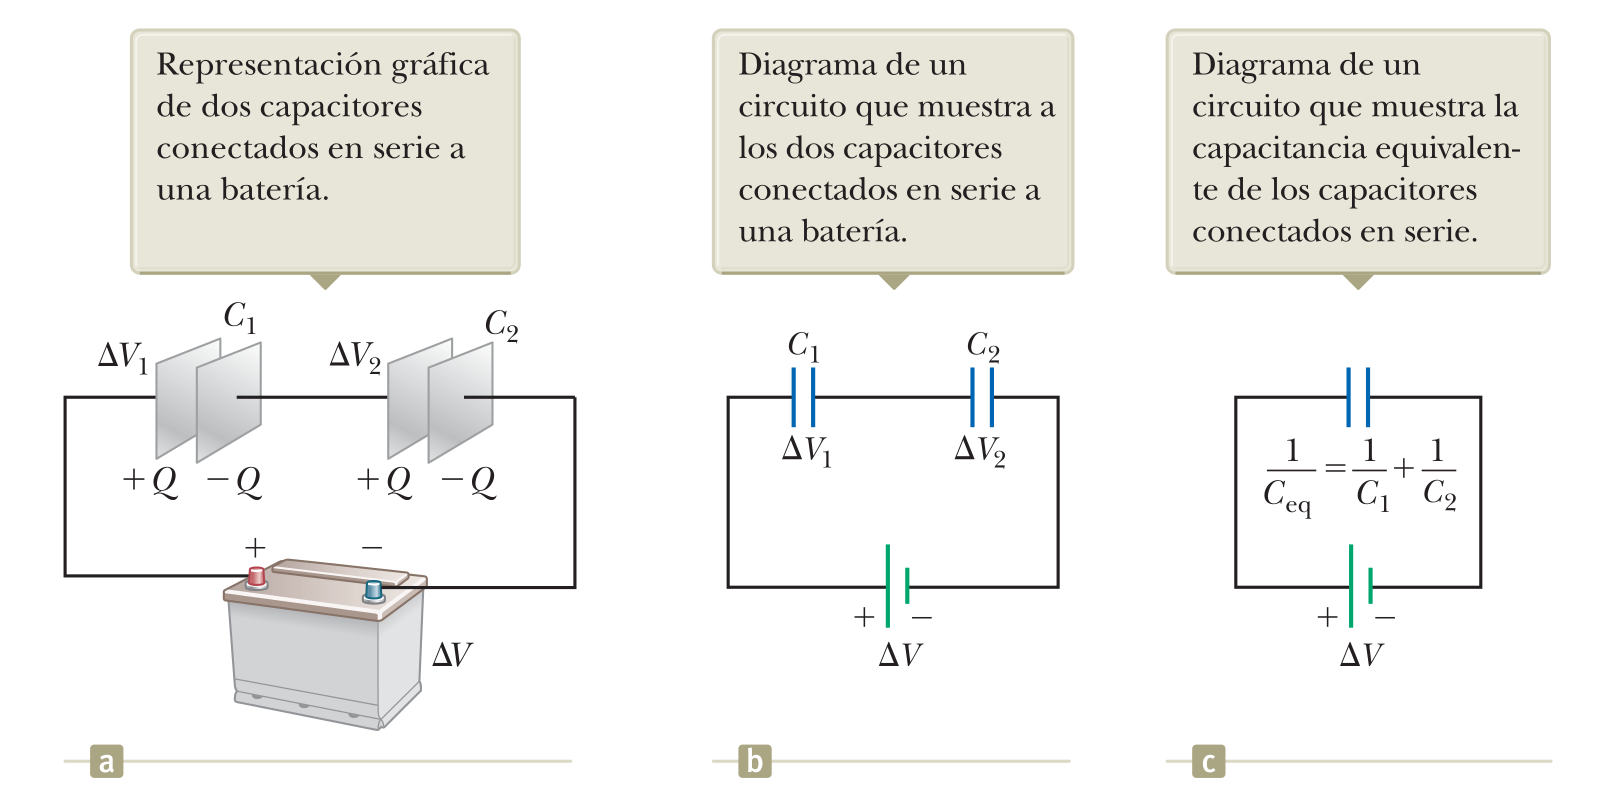
\includegraphics[width=0.9\textwidth]{capacitors_series.png}
    \caption{Configuración de capacitores en serie.}
    \label{fig:capacitors_series}
\end{figure}

\textbf{Configuración:} Todos los capacitores están conectados uno tras otro, por lo tanto, la misma carga \( Q \) pasa por todos. Es decir:

\[
Q_1 = Q_2 = \dots = Q_n = Q
\]

¿Por qué? Porque la carga del capacitor más pequeño actua como ``cuello de botella'' resultando en que la carga total es la misma en todos los capacitores.
\begin{figure}[ht]
    \centering
    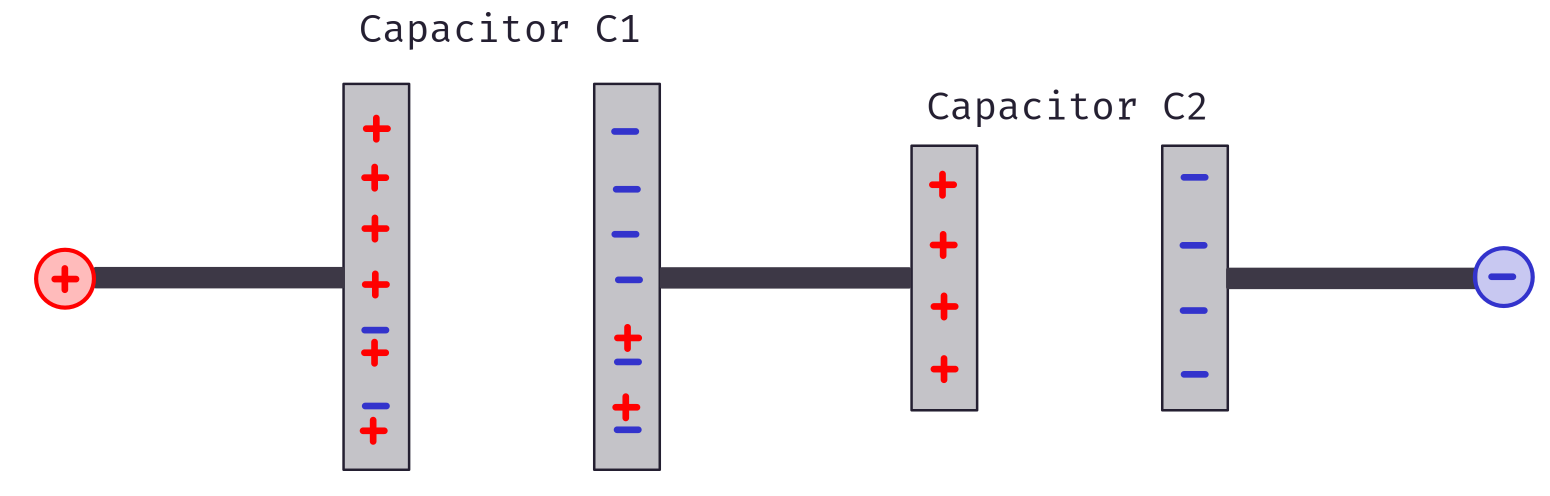
\includegraphics[width=0.9\textwidth]{capacitor_series_charge.png}
    \caption{La carga en ambos capacitores es la misma.}
    \label{fig:capacitors_series_charge}
\end{figure}

Como se puede ver en la figura \ref{fig:capacitors_series_charge}, la carga en ambos capacitores es la misma porque el capacitor \(C_2\) (más pequeño) está completamente cargado, esto provoca que el capacitor \(C_1\) (más grande) se vea limitado y no se use toda la capacidad. Esto es así porque los electrones se mueven de la placa izquierda del capacitor \(C_1\) a la placa derecha del capacitor \(C_2\). Cuando el capacitor \(C_2\) se carga completamente no puede acumular más carga. Por otro lado el capacitor \(C_1\) aún tiene electrones en su placa izquierda, pero estos electrones no tienen a donde ir, por lo que no se puede acumular más carga. Lo mismo sucede en las placas del medio de ambos capacitores. En una configuración en serie, la carga del capacitor más pequeño será la carga total usada de la batería.

Como la carga en todos los capacitores es la misma, la diferencia de potencial entre las placas de cada capacitor será diferente. La diferencia de potencial total es la suma de las diferencias de potencial individuales:

\[
V_{\text{total}} = V_1 + V_2 + \dots + V_n
\]

Pero \( V_i = \frac{Q}{C_i} \), entonces:

\[
V_{\text{total}} = \frac{Q}{C_1} + \frac{Q}{C_2} + \dots + \frac{Q}{C_n} = Q \left( \frac{1}{C_1} + \frac{1}{C_2} + \dots + \frac{1}{C_n} \right)
\]

Por definición, \( V_{\text{total}} = \frac{Q}{C_{\text{eq}}} \), así que:

\[
\frac{Q}{C_{\text{eq}}} = Q \left( \frac{1}{C_1} + \frac{1}{C_2} + \dots + \frac{1}{C_n} \right)
\]

Dividiendo ambos lados por \( Q \neq 0 \):

\[
\frac{1}{C_{\text{eq}}} = \frac{1}{C_1} + \frac{1}{C_2} + \dots + \frac{1}{C_n}
\]

\textbf{Resultado:} La inversa de la capacitancia equivalente en serie es igual a la suma de las inversas de las capacitancias individuales.

\begin{equation}
    \boxed{\frac{1}{C_{\text{total}}} = \frac{1}{C_1} + \frac{1}{C_2} + \frac{1}{C_3} + \ldots}
    \label{eq:capacitance_series}
\end{equation}
donde \( C_1, C_2, C_3, \ldots \) son las capacitancias individuales de los capacitores conectados en serie.